\documentclass[10pt,a4paper]{article}
\usepackage[utf8]{inputenc}
\usepackage{graphicx}
\usepackage[top=1in, bottom=1.25in, left=0.75in, right=0.75in]{geometry}

\title{projet-Electronique-Q1}
\author{Bronchain Olivier \\ Schellekens Vincent}
\date{\today}

\begin{document}
\maketitle

\section{Report}
\subsection{Block Scheme}
    In order to implement our game we will use the block scheme in Figure \ref{Block}. \\
    \begin{figure}[h!]
        \centering
        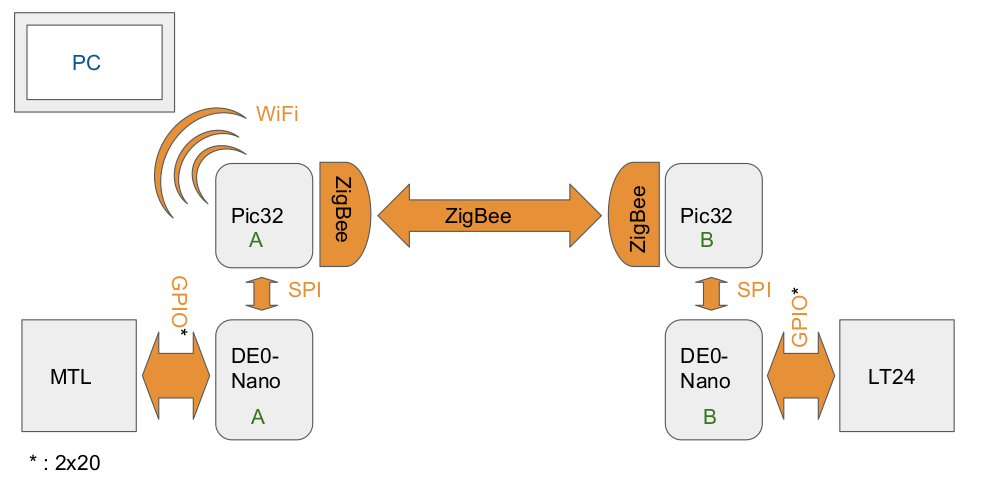
\includegraphics[width = 0.8 \textwidth]{lol3.png}
        \caption{Complete block scheme \label{Block}}
    \end{figure}
    During the game, the following teps are followed:
    \begin{itemize}
        \item \texttt{Before the round:}
		\begin{itemize}
			\item A and B are independent. The DE0-Nano A communicate via SPI with the PIC32 A (resp. B).
			\item A and B also communicate with their own screen. 
			\item A and B display a message mentioning that they are waiting the new round
			\item When A received a message from user asking for a new round, A send this information to PC and B to start the new round.
		\end{itemize}
        \item \texttt{During the round:}
		\begin{itemize}
			\item A and B are independent.
			\item A send message via WiFi to PC to update his behaviour.
			\item When a new fight occurs, A send a message to B with information like pv etc.   
		\end{itemize}
        \item \texttt{During a fight:}
		\begin{itemize}
			\item A send a message to be for the beginning of the round.
			\item A and B start a timer (timerA and timerB). A start it when he send the message  and B when he receive it. 
			\item When A and B finish the fight,  they each stop the timer and send it to the other user. The winner it the user with the smallest timer. 
			\item At the end of the fight, A send a message via Wifi to PC to update his behaviour
        	\end{itemize}
	\item \texttt{At the end of the round:}
			\begin{itemize}
			\item A send a message to B and PC to advertise the end of the round. 
			\end{itemize}
    \end{itemize}
   
\newpage
\section{Cahier des charges}
 
\end{document}
